% !TEX program = xelatex
% Beamer 样张：正二十面体群 / 正八面体群（8 帧，含公式、表格、TikZ、分步 overlay）
% 编译：xelatex -interaction=nonstopmode -halt-on-error sample.tex
\documentclass[aspectratio=169,10pt,fontset=none]{ctexbeamer}

% ---------- 中英文字体 ----------
\usepackage{fontspec}
\setCJKmainfont{Microsoft YaHei}
\setCJKsansfont{Microsoft YaHei}
\setCJKmonofont{Consolas}

% ---------- 数学与图形 ----------
\usepackage{amsmath,amssymb}
\usepackage{booktabs}
\usepackage{tikz}
\usetikzlibrary{arrows.meta,positioning,calc}

% ---------- 配色（与 PPTX 版一致） ----------
\definecolor{ink}{HTML}{1F3864}
\definecolor{accent}{HTML}{C00000}
\definecolor{gold}{HTML}{BF8F00}
\definecolor{greenink}{HTML}{2E6B2E}

\usetheme{default}
\usecolortheme[named=ink]{structure}
\setbeamertemplate{navigation symbols}{}
\setbeamertemplate{footline}[frame number]
\setbeamertemplate{itemize items}[circle]
\setbeamercolor{block title}{bg=ink!12,fg=ink}
\setbeamercolor{block body}{bg=ink!4,fg=black}
\setbeamercolor{block title alerted}{bg=accent!12,fg=accent}
\setbeamercolor{block body alerted}{bg=accent!4,fg=black}
\setbeamercolor{block title example}{bg=greenink!12,fg=greenink}
\setbeamercolor{block body example}{bg=greenink!5,fg=black}
\setbeamertemplate{frametitle}{\vskip4pt\insertframetitle\par\vskip2pt%
  \textcolor{accent}{\rule{\textwidth}{0.8pt}}\vskip-4pt}

\title{正二十面体群与正八面体群}
\subtitle{Beamer 样张 \;·\; $I\cong A_5$ 与 $O\cong S_4$}
\author{exercise\_abstract 库}
\date{\today}

\begin{document}

% ---------------------------------------------------------------- 1 标题页
\begin{frame}[plain]
  \titlepage
  \begin{center}
    \small 同一份内容、同一套配色：这里用 \LaTeX{} 排版，数学是可选中文本
  \end{center}
\end{frame}

% ------------------------------------------------------------ 2 群总览表
\begin{frame}[t]{三个旋转群总览}
  \begin{table}
    \centering
    \begin{tabular}{llrrl}
      \toprule
      群 & 抽象同构 & 阶 & 共轭类数 & 不可约特征标维数 \\
      \midrule
      $T$（正四面体）   & $A_4$ & 12 & 4 & $1,1,1,3$ \\
      $O$（正八面体）   & $S_4$ & 24 & 5 & $1,1,2,3,3$ \\
      $I$（正二十面体） & $A_5$ & 60 & 5 & $1,3,3,4,5$ \\
      \bottomrule
    \end{tabular}
  \end{table}
  \vspace{0.4em}
  \begin{alertblock}{全对称群（允许反射）}
    正四面体 $\cong S_4$（24）；立方体/正八面体 $\cong S_4\times C_2$（48）；
    正十二面体/正二十面体 $\cong A_5\times C_2$（120）。
  \end{alertblock}
\end{frame}

% ------------------------------------------- 3 题面 + 分步解答（overlay）
\begin{frame}[t]{G203 · 正八面体群的类方程与正规子群}
  \begin{block}{题面（Artin \textit{Algebra} 2e, Ch.~7, §4, Ex.~4.5, 印刷 p.~223 / PDF p.~235）}
    (a) 求正八面体群 $O$ 的类方程。\quad
    (b) 它含两个真正规子群：找出它们、证明它们正规，并证明没有别的。
  \end{block}
  \vspace{0.2em}
  \begin{enumerate}[<+->]
    \item 由 $O\cong S_4$，共轭类按轮换型分类，类大小为 $1,6,3,8,6$，故
      \[ 24=1+6+3+8+6. \]
    \item $A_4=\ker(\operatorname{sgn})$ 阶为 $12$；$V_4=\{1,(12)(34),(13)(24),(14)(23)\}$ 是单位元类与双对换类之并，两者都正规。
    \item 正规子群必是含 $1$ 的共轭类之并，其阶整除 $24$；在 $1,6,3,8,6$ 中检查，只有
      \[ 1+3=4,\qquad 1+3+8=12. \]
    \item \alert{结论}：真非平凡正规子群恰为 $V_4$ 与 $A_4$。
  \end{enumerate}
  \note{这一帧有 4 个 overlay 步骤：PDF 演讲版会展开成 4 页，handout 版压回 1 页。}
\end{frame}

% -------------------------------------------- 4 特征标表 + 置换分解公式
\begin{frame}[t]{Rep80 · $O\cong S_4$ 的特征标表与置换分解}
  \[
    \begin{array}{c|rrrrr}
                 & 1 & (12) & (12)(34) & (123) & (1234) \\ \hline
      1          & 1 & 1  & 1  & 1  & 1  \\
      \varepsilon& 1 & -1 & 1  & 1  & -1 \\
      \tau       & 2 & 0  & 2  & -1 & 0  \\
      \sigma     & 3 & 1  & -1 & 0  & -1 \\
      \sigma\varepsilon & 3 & -1 & -1 & 0 & 1
    \end{array}
  \]
  \vspace{-0.4em}
  \begin{align*}
    \mathbb{C}[\text{面}]           &= 1\oplus\tau\oplus\sigma\varepsilon, &
    \mathbb{C}[\text{顶点}]         &= 1\oplus\varepsilon\oplus\sigma\oplus\sigma\varepsilon,\\
    \mathbb{C}[\text{对径棱}]       &= 1\oplus\tau\oplus\sigma, &
    \mathbb{C}[\text{内接正四面体}] &= 1\oplus\varepsilon.
  \end{align*}
  \begin{exampleblock}{维数核对}
    面 $1+2+3=6$；顶点 $1+1+3+3=8$；对径棱 $1+2+3=6$；内接正四面体 $1+1=2$。
  \end{exampleblock}
\end{frame}

% --------------------------------------------------- 5 TikZ：内接正四面体
\begin{frame}[t]{G184/G204 · 立方体中的两个内接正四面体}
  \begin{columns}[T]
    \begin{column}{0.48\textwidth}
      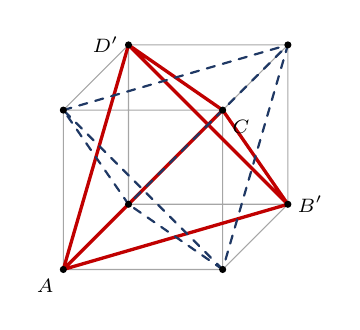
\begin{tikzpicture}[scale=0.92,line join=round,line cap=round,>=Stealth]
        \coordinate (A) at (0,0);     \coordinate (B) at (2.2,0);
        \coordinate (C) at (2.2,2.2); \coordinate (D) at (0,2.2);
        \coordinate (A') at (0.9,0.9);   \coordinate (B') at (3.1,0.9);
        \coordinate (C') at (3.1,3.1);   \coordinate (D') at (0.9,3.1);
        % 立方体
        \draw[gray!70] (A)--(B)--(C)--(D)--cycle
                       (A')--(B')--(C')--(D')--cycle
                       (A)--(A') (B)--(B') (C)--(C') (D)--(D');
        % 四面体 I：偶顶点 A, C, B', D'
        \draw[accent,very thick] (A)--(C)--(B')--(D')--cycle (A)--(B') (C)--(D');
        % 四面体 II：奇顶点 B, D, A', C'
        \draw[ink,thick,dashed] (B)--(D)--(A')--(C')--cycle (B)--(A') (D)--(C');
        \foreach \p in {A,B,C,D,A',B',C',D'} \fill[black] (\p) circle (1.4pt);
        \node[below left,font=\scriptsize] at (A) {$A$};
        \node[below right,font=\scriptsize] at (C) {$C$};
        \node[left,font=\scriptsize] at (D') {$D'$};
        \node[right,font=\scriptsize] at (B') {$B'$};
      \end{tikzpicture}
    \end{column}
    \begin{column}{0.50\textwidth}
      \begin{block}{题面（Ch.~6, §12, Ex.~12.4）}
        设 $G=O$ 是立方体的旋转群，$H$ 是把两个内接正四面体之一映到自身的子群，证明 $H=T$。
      \end{block}
      \begin{enumerate}[<+->]
        \item 8 个顶点按坐标和的奇偶分成两个正四面体（红、蓝），四分之一转交换它们。
        \item 故 $O$ 在这二元集上传递，$[O:H]=2$，$|H|=12$。
        \item 每个四面体旋转同时是立方体旋转：$T\le H$。
        \item $|T|=12=|H|$，于是 $H=T\cong A_4$。
      \end{enumerate}
    \end{column}
  \end{columns}
\end{frame}

% ------------------------------------------------- 6 TikZ：A5 的子群格
\begin{frame}[t]{G186 · $I\cong A_5$ 的子群型（含个数）}
  \centering
  \begin{tikzpicture}[scale=0.88,>=Stealth,
      box/.style={draw=ink,rounded corners=2pt,inner sep=2.4pt,font=\small,fill=ink!4},
      lab/.style={font=\scriptsize,text=ink}]
    \node[box] (A5)  at (0,4.3)   {$A_5$};
    \node[box] (A4)  at (-3.5,2.9){$A_4$};
    \node[box] (D5)  at (0,2.9)   {$D_5$};
    \node[box] (D3)  at (3.5,2.9) {$D_3$};
    \node[box] (V4)  at (-3.7,1.6){$V_4$};
    \node[box] (C3)  at (-1.1,1.6){$C_3$};
    \node[box] (C5)  at (1.3,1.6) {$C_5$};
    \node[box] (C2)  at (0.3,0.3) {$C_2$};
    \node[box] (tr)  at (0.3,-0.9){$\{1\}$};
    \draw (A5)--(A4); \draw (A5)--(D5); \draw (A5)--(D3);
    \draw (A4)--(V4); \draw (A4)--(C3);
    \draw (D3)--(C3); \draw (D3)--(C2);
    \draw (D5)--(C5); \draw (D5)--(C2);
    \draw (V4)--(C2); \draw (C3)--(C2); \draw (C5)--(D5);
    \draw (C2)--(tr);
    \node[lab] at (-4.3,3.15) {$5$ 个};
    \node[lab] at (0.95,3.42)  {$6$ 个};
    \node[lab] at (4.15,3.15) {$10$ 个};
    \node[lab] at (-4.35,1.85){$5$ 个};
    \node[lab] at (-1.1,1.95) {$10$ 个};
    \node[lab] at (1.75,1.95) {$6$ 个};
    \node[lab] at (1.1,0.45)  {$15$ 个};
  \end{tikzpicture}
  \vspace{0.1em}
  \begin{block}{}
    循环群由旋转生成；$V_4$ 来自内接正四面体；$D_3,D_5$ 是三重、五重轴的正规化子；
    $A_4$ 稳定一个内接正四面体。$T$ 侧为 $\{1\},C_2,C_3,V_4,A_4$。
  \end{block}
\end{frame}

% --------------------------------------------------- 7 输出形态与实测数据
\begin{frame}[t]{一份源，四种形态}
  \begin{itemize}
    \item \alert{演讲版}：\texttt{aspectratio=169}，overlay 逐步展开（本文件）。
    \item \alert{讲义版}：\texttt{handout} 选项，overlay 自动压平；\alert{讲者备注}用 \texttt{\textbackslash note\{...\}}。
    \item \alert{可读文章}：\texttt{beamerarticle} 出题解讲义；同一源也能出 reveal.js（MathJax）。
  \end{itemize}
  \vspace{0.2em}
  \begin{exampleblock}{本机实测（TeX Live 2023 + XeLaTeX）}
    \begin{tabular}{@{}ll@{}}
      演讲版页数 & \textbf{13}（7 帧，含 overlay 展开）\\
      讲义版页数 & \textbf{7}（同一源，overlay 压平）\\
      编译耗时   & 两次 \texttt{xelatex} 共 \textbf{6.7\,s} \\
      公式形态   & 可选中、可搜索的矢量文本，不需要 Unicode 改写
    \end{tabular}
  \end{exampleblock}
  \note{把 \texttt{sample.tex} 交给 \texttt{latexmk -xelatex} 即可；源文件可 Git diff。}
\end{frame}

\end{document}
